\clearpage

\section{Práctica 5: Sistema de iluminación por biestable}

\subsection{Introducción}
En esta práctica se configurará el encendido de un sistema de iluminación conectado directamente a corriente alterna suministrada
a través del uso de emisores infrarrojo, mediante un sistema de seguridad de encendido/apagado con un circuito integrado
llamado biestable, con la capacidad de guardar si está encendido o apagado como información en memoria.

\subsection{Objetivos}
Generar un sistema de interrupciones para encender y apagar un foco usando arreglos infrarrojos y biestables.


\subsection{Marco teórico}
\subsubsection{Biestables}
Los circuitos biestables, o también llamados Flip-Flops, son circuitos de dos estados o digitales que guarda la información
dada la manipulación de dos entradas. Para ser más precisos, funciona de tal manera que en la entrada 1 se active la información
de encendido o HIGH y la segunda se encargue de cambiar su estado a LOW o apagado. Una vez que entre señal a la activación, no
importa las veces que se apague la señal o se encienda en la terminal de entrada 1. Su estado no se puede cambiar a apagado mas
que al enviar una señal en la terminal de entrada 2, y este efecto ocurre cuando su estado es cero. 
\parencite{markovic2001analysis}

El diagrama de un biestable es el siguiente:

\begin{figure}
    \centering
    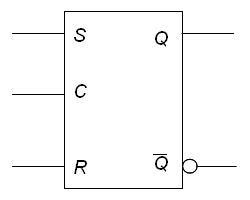
\includegraphics[scale=0.5]{media/Biestable.jpg}
    \caption{Biestable}
    \label{Fig: Circuito biestable}
\end{figure}

Las entradas se denominan SET y RESET que, como sus nombres indican, activan la memoria y regresan al estado inicial.
Otro detalle son las salidas, los cuales por defecto existen dos: salida directa \(Q\) y negada \(\overline{Q}\) para 
usarse en lógica inversa.

Este sencillo arreglo de memoria se llama Biestable asíncrono. Por otro lado, existe otro arreglo que incluye una quinta
terminal llamado síncrono, tal como se muestra en la imagen anterior. Contiene la terminal CLOCK el cual es usado para
permitir o no un cambio.

El más sencillo es del tipo D, el cual toma la estructura de un asíncrono para únicamente almacenar un bit de información.
Este tipo es conocido como tipo D. 

El circuito integrado a usar para esta practica tiene como nombre de modelo MC14013B, el cual contiene dos bietables tipo D, 
pero que además contiene la entrada de CLOCK. El diagrama se encuentra en la ilustración 2.

\begin{figure}
    \centering
    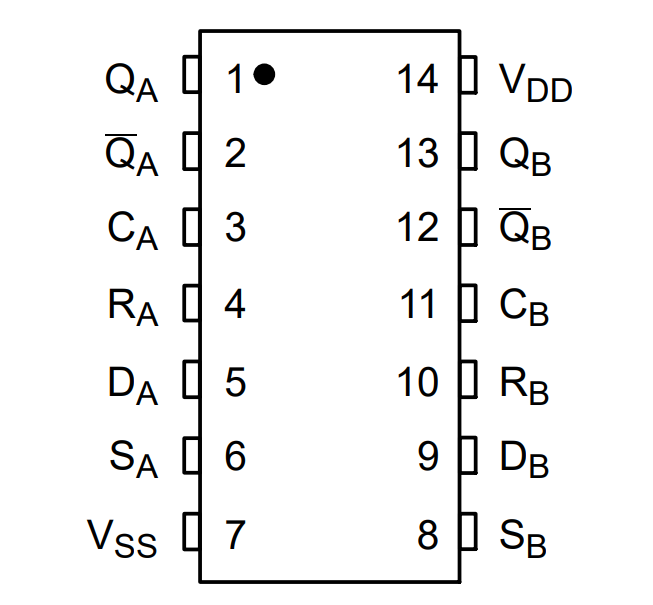
\includegraphics[scale=0.5]{media/MC14013B.png}
    \caption{Diagrama del biestable dual MC14013B}
    \label{Fig: Diagrama del biestable dual MC14013B}
\end{figure}

\subsubsection{Optoacopladores}
Los Optoacopladores son cirtuitos integrados que funcionan como interruptores mediante la saturación de un fototransistor
a través de un diodo LED. Usualmente se usan optoacopladores que tienen transistor de salidad un BJT, darlington o un triac.
El mayor uso para estos circuitos es del aislamiento siendo el único contacto entre los circuito que separa dicho arreglo
es la luz utilizada para activar el transistor. Con ello se puede manipular dos fuentes de voltaje o circuitos analógicos y 
digitales en un mismo sistema. \parencite{bera2012opto}

El optoacoplador utilizado para esta práctica es el MOC3011, el cual el transistor interno es un TRIAC, usado como interruptor
en corriente alterna y electrónica de potencia.

\begin{figure}
    \centering
    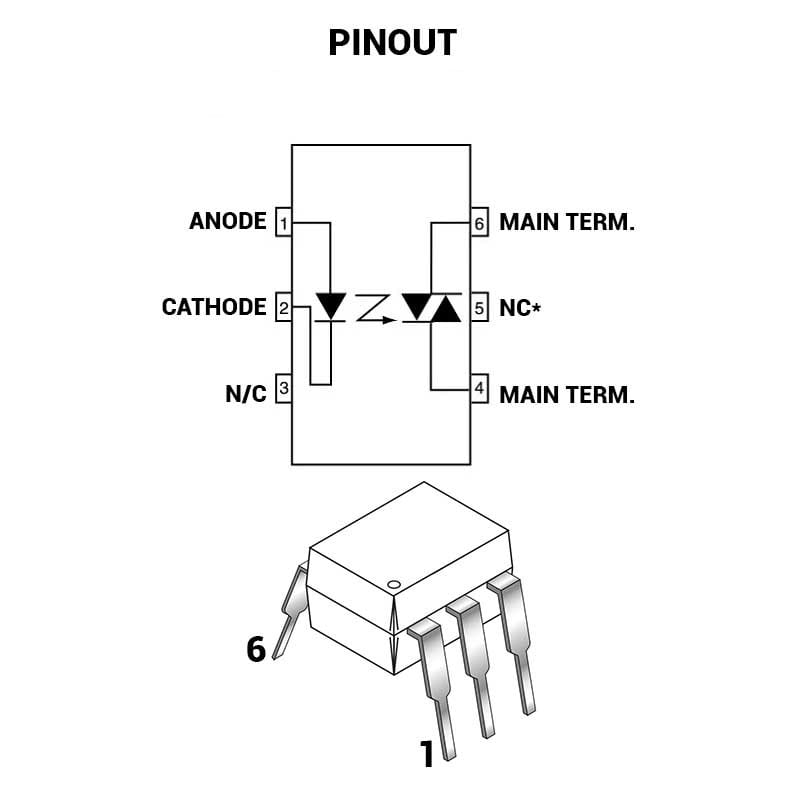
\includegraphics[scale=0.15]{media/MOC3011.jpg}
    \caption{Diagrama del optoacoplador TRIAC MOC3011}
    \label{Fig: Diagrama del optoacoplador TRIAC MOC3011}
\end{figure}


\subsection{Circuito}

El diagrama es el siguiente:

\begin{figure}[h]
    \centering
    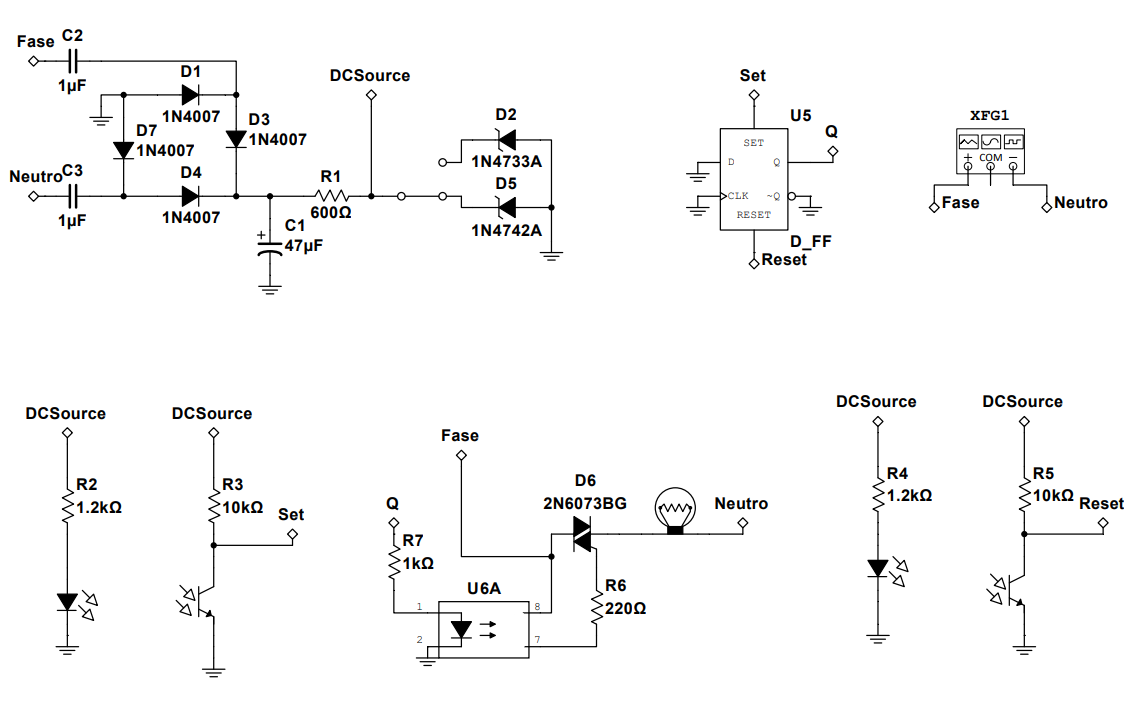
\includegraphics[scale=0.4]{media/Circuito.png}
    \caption{Diagrama de la práctica}
    \label{Fig: Diagrama de la práctica}
\end{figure}

Este circuito consta de 4 etapas: alimentación sin transformador (mencionado en la práctica anterior), entrada de información
mediante el sistema emisor/receptor infrarrojo, bajo un arreglo de reistencia pull up, el biestable, y la salida analógica.

En la etapa de entrada de información, se usan dos etapas de emisores infrarrojo que sustituye el uso de botones para 
fines específicos.

En el arreglo de salida al foco, se usa otro TRIAC el cual es el contacto directo con el cuministro del tomacorriente, puesto
que el TRIAC instalado en el optoacoplador servirá únicamente como interruptor lógico.


\subsection{Resultados}

\begin{figure}[h]
    \centering
    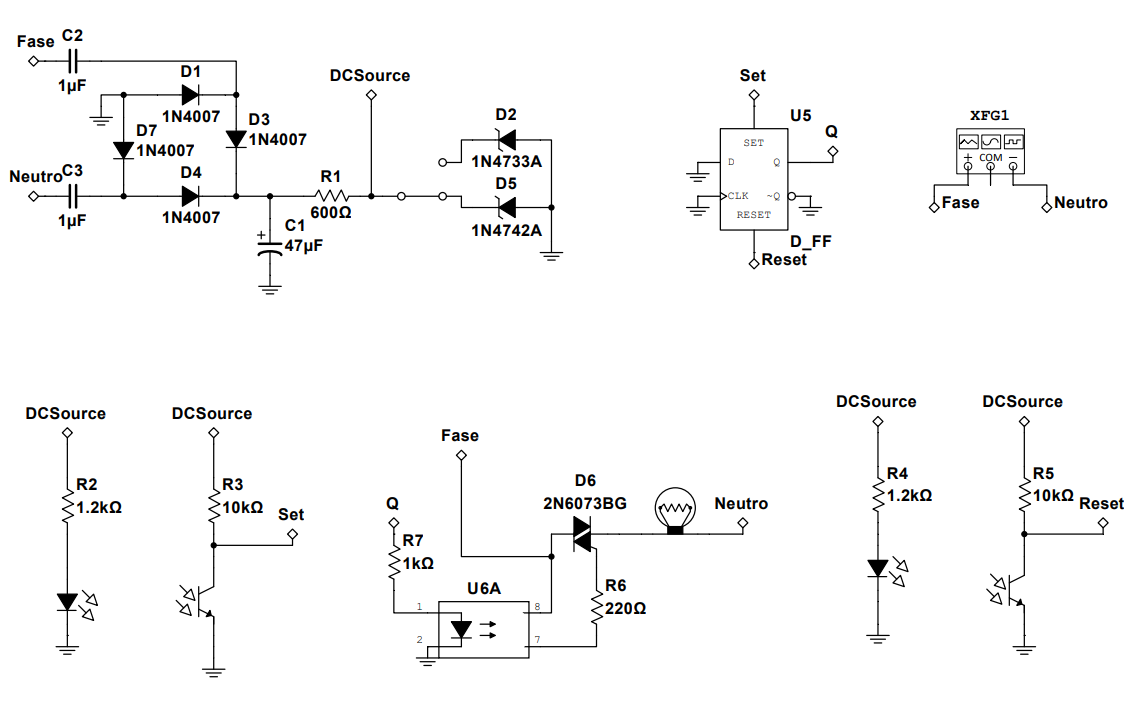
\includegraphics[scale=0.4]{media/Circuito.png}
    \caption{Circuito contruido}
    \label{Fig: Circuito contruido}
\end{figure}

El circuito cumple con sus funciones y no sufre de caída de voltaje al usarlo para este caso. Tal como muestran en las 
siguiente fotos.

\begin{figure}[h]
    \centering
    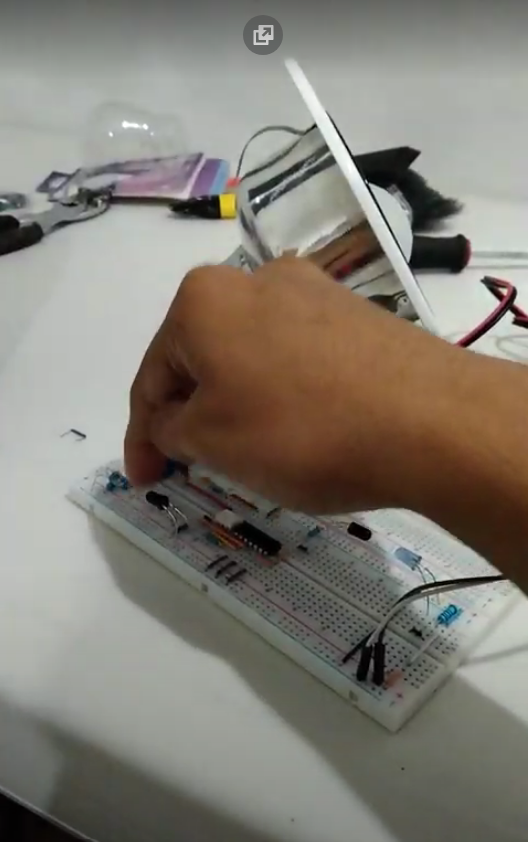
\includegraphics[scale=0.4]{media/Resultados1.png}
    \caption{Resultados de la práctica 1}
    \label{Fig: Resultados de la practica 1}
\end{figure}

\begin{figure}[h]
    \centering
    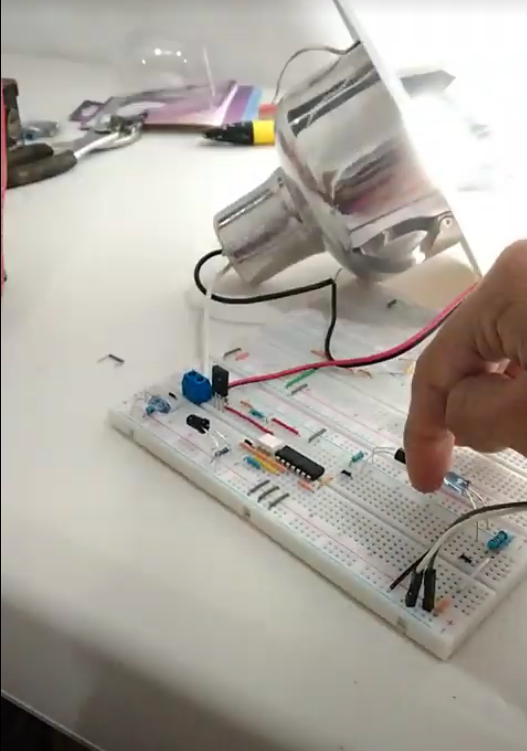
\includegraphics[scale=0.4]{media/Resultados2.png}
    \caption{Resultados de la práctica 2}
    \label{Fig: Resultados de la practica 2}
\end{figure}

\subsection{Conclusiones}

El arreglo de emisor/receptor infrarrojo funciona como interruptor para activar y desactivar circuitos.

Este arreglo puede utilizarse en sistemas de iluminación, audio, incluso para manipulación de datos y sistemas automáticos 
e industriales.

El biestable guarda en memoria el estado detectado por el SET o RESET y esto ayuda como un elemento de seguridad contra
reacciones del circuito no esperadas.
